\section{eo\-Assembled\-Fitness\-Best\-Stat$<$ EOT $>$ Class Template Reference}
\label{classeo_assembled_fitness_best_stat}\index{eoAssembledFitnessBestStat@{eoAssembledFitnessBestStat}}
Fitness values of best individuum in a population, where the fitness is of type eo\-Scalar\-Assembled\-Fitness.  


{\tt \#include $<$eo\-Assembled\-Fitness\-Stat.h$>$}

Inheritance diagram for eo\-Assembled\-Fitness\-Best\-Stat$<$ EOT $>$::\begin{figure}[H]
\begin{center}
\leavevmode
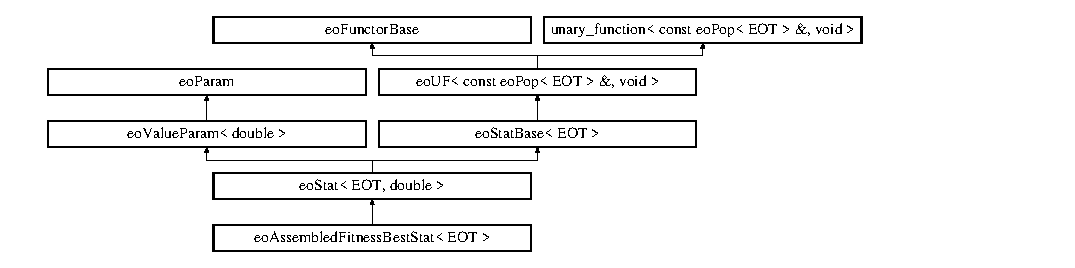
\includegraphics[height=3.15315cm]{classeo_assembled_fitness_best_stat}
\end{center}
\end{figure}
\subsection*{Public Types}
\begin{CompactItemize}
\item 
typedef EOT::Fitness {\bf Fitness}\label{classeo_assembled_fitness_best_stat_w0}

\end{CompactItemize}
\subsection*{Public Member Functions}
\begin{CompactItemize}
\item 
{\bf eo\-Assembled\-Fitness\-Best\-Stat} (unsigned \_\-which\-Term=0, std::string \_\-description=\char`\"{}Best Fitness\char`\"{})\label{classeo_assembled_fitness_best_stat_a0}

\item 
virtual void {\bf operator()} (const {\bf eo\-Pop}$<$ {\bf EOT} $>$ \&\_\-pop)\label{classeo_assembled_fitness_best_stat_a1}

\begin{CompactList}\small\item\em The pure virtual function that needs to be implemented by the subclass. \item\end{CompactList}\end{CompactItemize}
\subsection*{Private Attributes}
\begin{CompactItemize}
\item 
unsigned {\bf which\-Fitness\-Term}\label{classeo_assembled_fitness_best_stat_r0}

\end{CompactItemize}


\subsection{Detailed Description}
\subsubsection*{template$<$class EOT$>$ class eo\-Assembled\-Fitness\-Best\-Stat$<$ EOT $>$}

Fitness values of best individuum in a population, where the fitness is of type eo\-Scalar\-Assembled\-Fitness. 

Specify in the constructor, for which fitness term (index) the value should be evaluated. 



Definition at line 87 of file eo\-Assembled\-Fitness\-Stat.h.

The documentation for this class was generated from the following file:\begin{CompactItemize}
\item 
eo\-Assembled\-Fitness\-Stat.h\end{CompactItemize}
